\documentclass[final]{siamltex}
\usepackage{geometry}   % See geometry.pdf to learn the layout
                        % options.  There are lots.
\usepackage{graphicx}
\usepackage{epstopdf}
\usepackage{color,amsmath,latexsym,amsfonts,amssymb}
\usepackage{wrapfig}

\DeclareGraphicsRule{.tif}{png}{.png}{`convert #1 `dirname #1`/`basename #1 .tif`.png}

%-----Extra Formatting Options
\textheight 9.0truein
\textwidth 6.5truein
\addtolength{\topmargin}{-0.25in}
\addtolength{\evensidemargin}{-0.5in}
\setlength{\parindent}{0em}
\setlength{\parskip}{2ex}

%----My Definitions---
\renewcommand{\(}{\left(}
\renewcommand{\)}{\right)}
\newcommand{\dt}{\Delta t}
\newcommand{\R}{\mathrm R}
\newcommand{\N}{\mathrm N}
\newcommand{\alfven}{Alfv\'{e}n }
\newcommand{\sundials}{\normalfont\scshape Sundials}
\newcommand{\fninety}{\normalfont\scshape Fortran90}
\newcommand{\kinsol}{\normalfont\scshape KINSol}
\newcommand{\cvode}{\normalfont\scshape Cvode}
\newcommand{\openad}{\normalfont\scshape OpenAD}
\newcommand{\hypre}{\normalfont\scshape Hypre}
\newcommand{\superlu}{\normalfont\scshape SuperLU}
\newcommand{\petsc}{\normalfont\scshape PETSc}
\newcommand{\tao}{\normalfont\scshape TAO}
\newcommand{\trilinos}{\normalfont\scshape Trilinos}
\newcommand{\bbeta}{{\bf \beta}}
\newcommand{\bU}{{\bf U}}
\newcommand{\tU}{{\tilde{\bf U}}}
\newcommand{\bV}{{\bf V}}
\newcommand{\bW}{{\bf W}}
\newcommand{\bF}{{\bf F}}
\newcommand{\bG}{{\bf G}}
\newcommand{\bH}{{\bf H}}
\newcommand{\bS}{{\bf S}}
\newcommand{\pt}{\tilde{p}}
\newcommand{\tbF}{\tilde{\bF}}
\newcommand{\tbG}{\tilde{\bG}}
\newcommand{\tbH}{\tilde{\bH}}
\newcommand{\mI}{{\mathcal I}}
\newcommand{\mJ}{{\mathcal J}}
\newcommand{\mR}{{\mathcal R}}
\newcommand{\bu}{{\bf u}}
\newcommand{\bB}{{\bf B}}

%----Head Matter-------------------------------------------
\title{Quantum Algorithms for Numerical Methods} 
\author{Micah A. Thornton \& Daniel R.~Reynolds\\
  (Two Semester Project)
} 
%\email{mathornton@smu.edu, reynolds@smu.edu}
%\date{April 10, 2015}

%----Begin Document----------------------------------------
\begin{document}

\maketitle

\pagestyle{myheadings}
\thispagestyle{plain}
\mark{M.A.~Thornton \& D.R.~Reynolds -- Quantum Algos. for Numerical Methods}


\section{Introduction}
\label{sec:intro}
At the precipice of computation sits a golden fleece of the modern era. Quantum Computation is a buzz word in academia, and industry alike. Those who misunderstand this theoretical machine 
herald it as an end-all that will solve all the modern problems in complexity theory. Those who understand it's power are able to approach it rationally, and determine which problems it 
can solve with increased efficiency compared with it's modern Turing alternative. At the end of the day there are some problems for which the doped silicon of electronic computers simply outperforms the polarized glass of their quantum companions. it is up to those with a theoretical understanding of the mathematical, and physical properties of the proposed machine to determine where beneficiary algorithms might overlap and allow for substantial speed up using this new paradigm of Quantum Computation.


\section{Problem Description}
\label{sec:problem}
The heart of this project lies with the desire to understand whether or not certain methods from traditional numerical analysis can experience a theoretical (and experimental by use of a quantum simulator)

\section{Solution Approach}
\label{sec:solvers}
There are primarily two forms of computer logic (Sequential and
Combinational). Traditional in electronic computers, sequential logic
requires the use of memory elements, which are not available on
quantum computers. However, for algorithms that do require extensive
use of memory, we will create mixed signal digital-quantum circuits,
which can contain memory elements, while also making use of quantum
computation.  Combinational logic on the other hand does not require
memory elements, and simply propagates input values into output
responses. 

\begin{wrapfigure}{R}{0.5\textwidth}
  \begin{center}
    \begin{tabular}{|c|c||c|c|}
      \hline
      a & b & sum & carry-out \\
      \hline 
      0&0&0&0 \\
      0&1&1&0 \\
      1&0&1&0 \\
      1&1&0&1 \\
      \hline
    \end{tabular}
  \end{center}
\end{wrapfigure}
A primary goal of this project is to refine a tool that Micah Thornton
has already constructed which can handle the synthesis of quantum
designs given a verilog specification has already been developed.  
Verilog is a computer-aided-circuit design description language,
meaning it is used to specify the functionality of circuits before
they are fabricated.  

The diagram below represents how the tool works when provided a purely
combinational specification of a simple single half-adder -- an
electronic circuit that adds two bits together, the 
truth table for this circuit is given above.  By using the quantum
synthesis tool we were able to extract the transfer matrix for this
logical operation and convert it into a quantum circuit
description.  This is a very small example, but it illustrates the
power of the tool, that performed this conversion automatically. 
\begin{center}
  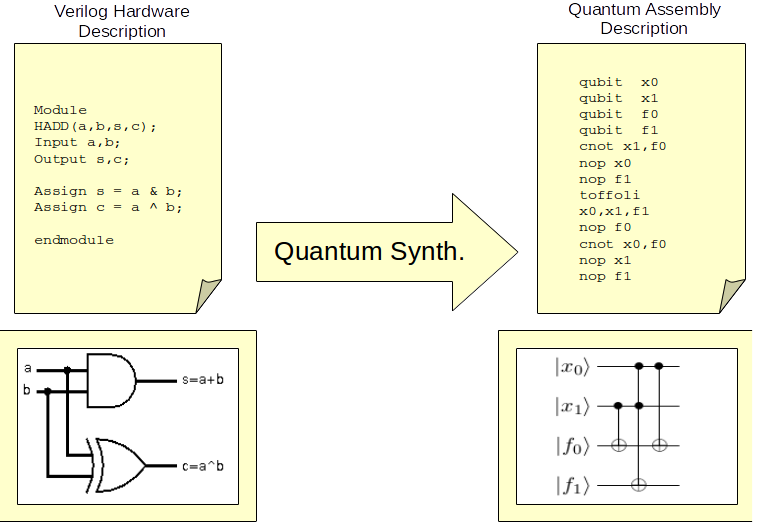
\includegraphics[scale=0.55]{QuantumSynthesis.png}
\end{center}
Within this project, we will upgrade this tool
so that it may automatically synthesize verilog descriptions of
numerical methods into their equivalent quantum forms.  With this
tool, we may then implement target numerical methods in computational
logic and automatically convert these into their quantum computing
equivalent.  Once these have been created, we will use existing
quantum simulators to test these algorithms and evaluate their promise
in quantum computing. 



\section{Personnel}
\label{sec:sam}
No project would be succesful without a dedicated team of people to work on it, and this is no exception. 

Micah Thornton is a dedicated student, who is pursuing three degrees in Mathematics, Statistics, and Computer Engineering, as well as a masters in Electrical Engineering. Having already succesfully completed a Quantum Computing course, as well as upper level math, and computer science classes, Micah is eager to get underway with this project. 

%%%%%%%%%%%

\bibliography{ham2015}
\bibliographystyle{siam}

%%%%%%%%%%%

\end{document}
